% 赋范空间：范数与距离；收敛、极限与连续性；有限维赋范空间的性质（范数等价、完备性、级数、矩阵范数、对偶范数、商范数），只讨论有限维情形。

\section{范数与距离}
\label{sec:ls-normed-spaces}

用多项式近似一个函数时，要估计误差有多大；迭代产生一列近似时，要判断它是否趋于某个对象。这些问题都需要先规定向量的大小。第~\ref{chap:linear-operations}章用$\ell_1$、$\ell_2$、$\ell_\infty$范数度量$\mathbb R^d$中数组的大小，本节把这种度量推广到一般线性空间。

本节先给出范数的公理和例子，这一部分只用到线性运算与标量不等式；坐标范数之间的比较已在第~\ref{sec:ls-error-scale-comparison}节给出。然后证明有限维空间中任意两个范数等价，此后的开集、闭集、收敛、极限与连续性因而都不依赖所选范数；第~\ref{sec:ls-derived-norms}节再在矩阵、线性泛函和商空间上定义范数。本章只讨论有限维空间。

\subsection{范数的定义与示例}
\label{sec:ls-normed-space-definition}

\paragraph{范数的定义}
第~\ref{sec:ls-p-norm-properties}节证明了，$p$范数非负、正定、齐次，并满足三角不等式。这些性质只涉及加法和数乘，因此可以直接作为一般线性空间上“大小”的要求。
\begin{definition}[赋范空间]
\label{def:ls-normed-space}
\label{def:functional-normed-space}
设$V$是实线性空间。映射$\lVert\cdot\rVert:V\to[0,\infty)$若对任意$\bm x,\bm y\in V$与$c\in\mathbb R$满足
\begin{enumerate}
 \item 正定性：$\lVert\bm x\rVert=0$当且仅当$\bm x=\bm0$；
 \item 齐次性：$\lVert c\bm x\rVert=|c|\,\lVert\bm x\rVert$；
 \item 三角不等式：$\lVert\bm x+\bm y\rVert\leq\lVert\bm x\rVert+\lVert\bm y\rVert$，
\end{enumerate}
就称为$V$上的\term{范数}（norm）；配备范数的线性空间$(V,\lVert\cdot\rVert)$称为\term{赋范空间}（normed space）。
\end{definition}
范数诱导距离$d(\bm x,\bm y)=\lVert\bm x-\bm y\rVert$。这个距离非负，只在$\bm x=\bm y$时为零，对称，并满足$d(\bm x,\bm z)\leq d(\bm x,\bm y)+d(\bm y,\bm z)$。这四条正是度量空间对距离的要求，所以赋范空间是一类特殊的度量空间；一般度量空间可参考\BookChapterRef{chap:metric-spaces}{卷四“度量空间”一章}。它的距离还与线性运算相容：平移不改变距离，缩放按同一比例改变距离。

三角不等式还能反过来控制长度之差。把它用于$\bm x=(\bm x-\bm y)+\bm y$，得$\lVert\bm x\rVert-\lVert\bm y\rVert\leq\lVert\bm x-\bm y\rVert$；交换$\bm x,\bm y$，又得$\lVert\bm y\rVert-\lVert\bm x\rVert\leq\lVert\bm x-\bm y\rVert$。两式合起来就是反向三角不等式
\begin{equation}
 \bigl|\lVert\bm x\rVert-\lVert\bm y\rVert\bigr|\leq\lVert\bm x-\bm y\rVert.
 \label{eq:ls-reverse-triangle}
\end{equation}
即两个向量的长度之差不超过差向量的长度。下一节用它说明范数随向量收敛。

\paragraph{坐标范数是范数}
\label{sec:ls-norms-distances}
\label{sec:linear-algebra-distance-relations}
第~\ref{chap:linear-operations}章的$p$范数正是这一定义的例子。第~\ref{sec:ls-p-norm-properties}节已经证明，每个$p$范数非负、正定、齐次，并满足三角不等式（定理~\ref{thm:linear-algebra-minkowski}）。这恰好是定义~\ref{def:ls-normed-space}的三条要求，所以$\lVert\cdot\rVert_p$（$1\leq p\leq\infty$）是$\mathbb R^d$上的范数，$(\mathbb R^d,\lVert\cdot\rVert_p)$是赋范空间。

\paragraph{其他空间上的范数}
除$p$范数外，前面还出现过别的范数。同形矩阵上的Frobenius范数，就是把矩阵元素排成向量后的$2$范数；诱导矩阵范数将在第~\ref{sec:ls-matrix-norms}节定义并验证。

在一般线性空间上，最直接的做法是借助坐标。若$\lVert\cdot\rVert_\star$是$\mathbb R^d$上的范数，$\mathcal B$是$V$的基，则$\lVert\bm v\rVert=\lVert[\bm v]_{\mathcal B}\rVert_\star$是$V$上的范数，因为坐标映射是保持线性组合的双射。也可以不经过坐标，直接用对象本身的性质规定范数。下面在$P_k$上各举一例。
\begin{example}[多项式空间上的两个范数]
\label{ex:ls-polynomial-norms}
对$p=a_0+a_1t+\cdots+a_kt^k$，可以看系数，也可以看函数在区间$[0,1]$上的取值，由此得到两个规则：
\[
\begin{gathered}
p\mapsto\max_{0\leq j\leq k}|a_j|,\\
p\mapsto\lVert p\rVert_\infty=\max_{t\in[0,1]}|p(t)| .
\end{gathered}
\]

第一个规则正是坐标$(a_0,\ldots,a_k)$在基$(1,t,\ldots,t^k)$下的$\ell_\infty$范数，按上面借助坐标的方法，它是范数。第二个规则不经过坐标，需要逐条检验公理。齐次性在每个$t$处成立，取最大值后仍成立。对三角不等式，每个$t$都满足$|p(t)+q(t)|\leq|p(t)|+|q(t)|\leq\lVert p\rVert_\infty+\lVert q\rVert_\infty$，左侧再对$t$取最大值即可。正定性依赖多项式的代数性质：次数不超过$k$的非零多项式至多有$k$个根，不能在整个区间$[0,1]$上为零。

所以两个规则都是$P_k$上的范数。前者借助坐标，后者直接用函数值，检验时只需用到多项式本身的性质。
\end{example}

有时只关心向量的一部分信息。这时可以去掉正定性，只保留非负性、齐次性与三角不等式，得到的尺度称为\term{半范数}（seminorm）。半范数可能把两个不同的点判为距离为零。
\begin{example}[只看第一个坐标的半范数]
\label{ex:ls-seminorm-first-coordinate}
在$\mathbb R^2$上只用第一个坐标衡量大小，令$p(\bm x)=|x_1|$。半范数要求的三条性质都由实数绝对值的性质得到：$p(\bm x)\geq0$，$p(c\bm x)=|cx_1|=|c|\,p(\bm x)$，并且$p(\bm x+\bm y)=|x_1+y_1|\leq|x_1|+|y_1|=p(\bm x)+p(\bm y)$。缺少的是正定性：非零向量$(0,1)^\top$满足$p\bigl((0,1)^\top\bigr)=0$。

因此$p$是半范数而不是范数。用它度量距离时，$(0,0)^\top$与$(0,1)^\top$的距离为$p\bigl((0,-1)^\top\bigr)=0$，两个不同的点被视为没有差别，第二个坐标上的差别完全被忽略。
\end{example}
因此使用半范数之前，须先说明哪些差别被有意忽略。

\subsection{有限维范数等价}
\label{sec:multivariable-norm-equivalence}
\label{sec:linear-algebra-sequence-convergence}
\phantomsection
\label{sec:ls-finite-dimensional-normed-properties}

上一小节与第~\ref{chap:linear-operations}章给出了许多范数，误差分析也常常在$\ell_1$、$\ell_2$、$\ell_\infty$与诱导矩阵范数之间切换。同一个向量在不同范数下的大小不同；那么，“接近”“收敛”“连续”这些说法会不会随范数改变？本小节证明，在有限维空间中不会：任意两个范数只相差常数倍。后面各节因此可以在任意范数下定义开集、收敛与连续性。

\begin{theorem}[有限维范数等价]
\label{thm:ls-norm-equivalence}
有限维实线性空间上任意两个范数$p,q$都等价：存在常数$c,C>0$，使$c\,q(\bm x)\leq p(\bm x)\leq C\,q(\bm x)$对所有$\bm x$成立。
\end{theorem}
\begin{proof}
零维空间只有零向量，结论显然；下设$\dim V=d\geq1$。思路是把每个范数都与一个固定的参照比较。固定基$(\bm b_1,\ldots,\bm b_d)$，把$\bm x=\sum_jx_j\bm b_j$等同于坐标向量$(x_1,\ldots,x_d)^\top$，取坐标的欧氏长度$\lVert\bm x\rVert_c=(\sum_jx_j^2)^{1/2}$作参照。

上界。对任意范数$p$，由三角不等式、齐次性与$p=q=2$的Hölder不等式，
\[
 \begin{gathered}
 p(\bm x)=p\Bigl(\sum_jx_j\bm b_j\Bigr)\leq\sum_j|x_j|\,p(\bm b_j)\leq C_p\lVert\bm x\rVert_c,\\
 C_p=\Bigl(\sum_jp(\bm b_j)^2\Bigr)^{1/2}.
 \end{gathered}
\]
下界。只需找到$m_p>0$，使$p(\bm x)\geq m_p\lVert\bm x\rVert_c$对一切$\bm x$成立。若不然，对每个正整数$n$都有$\bm x_n\neq\bm0$满足$p(\bm x_n)<\lVert\bm x_n\rVert_c/n$；由齐次性，可以设$\lVert\bm x_n\rVert_c=1$，于是$p(\bm x_n)<1/n$。这时每个坐标都满足$|x_{n,j}|\leq1$，坐标组成的实数列都有界。由实数列的Bolzano--Weierstrass定理，先从第一个坐标中选出收敛子列，再在这个子列中从第二个坐标选出收敛子列，如此进行$d$次，得到一个子列（仍记为$\bm x_n$），它的每个坐标都收敛：$x_{n,j}\to x_j$。令$\bm x=\sum_jx_j\bm b_j$。

这个极限$\bm x$引出矛盾。一方面，$\lVert\bm x_n-\bm x\rVert_c^2=\sum_j(x_{n,j}-x_j)^2$是有限个趋于零的数之和，所以$\lVert\bm x_n-\bm x\rVert_c\to0$；又$\lVert\bm x\rVert_c^2=\sum_jx_j^2=\lim_n\sum_jx_{n,j}^2=1$，所以$\bm x\neq\bm0$。另一方面，由三角不等式与上界，
\[
 p(\bm x)\leq p(\bm x_n)+p(\bm x-\bm x_n)<\frac1n+C_p\lVert\bm x_n-\bm x\rVert_c\to0,
\]
于是$p(\bm x)=0$，与范数的正定性矛盾。合起来，
\begin{equation}
 m_p\lVert\bm x\rVert_c\leq p(\bm x)\leq C_p\lVert\bm x\rVert_c.
 \label{eq:linear-algebra-finite-norm-equivalence}
\end{equation}

最后比较$p$与$q$：$p\leq C_p\lVert\cdot\rVert_c\leq(C_p/m_q)\,q$；交换$p,q$的角色，得反向不等式。
\end{proof}
定理中的常数依赖维数与所选范数，示例~\ref{ex:ls-l1-linf-constants}说明$\ell_1$与$\ell_\infty$之间的常数$1$与$d$不能改进。证明中真正依赖有限维的是下界：逐个坐标抽取收敛子列只能进行有限次。证明只用到实数列的Bolzano--Weierstrass定理（可参考\BookChapterRef{chap:limits-continuity}{卷一“极限与连续”一章}），不需要后面的收敛与连续性理论。

范数等价说明，后面各节的定性概念都与所选范数无关：开集、闭集与有界集（第~\ref{sec:multivariable-open-closed-sets}节），序列的收敛、柯西性与完备性，映射的极限与连续性，换一种范数都不改变；各节在定义处具体说明。不变的只是这些定性结论。数值误差与比较常数会随范数改变，常数还依赖维数，维数增长时不能视为统一的界。范数等价也不给出衰减速度：同一个收敛序列在一种范数下单调下降，在另一种范数下可能先上升。速度要在选定的范数中由具体结构估计。

\section{开集、闭集与有界集}
\label{sec:multivariable-open-closed-sets}

讨论收敛、极限与连续性时，先要说明点在什么样的集合里变化：基点周围是否留有向各个方向移动的余地，集合是否包含它边界上的点，集合是否伸向无穷远。这三个问题分别由开集、闭集与有界集回答。本节设$V$是有限维赋范空间，范数记为$\lVert\cdot\rVert$；例子取欧氏范数下的$\mathbb R^d$或Frobenius范数下的矩阵空间。由上一节的范数等价，这些概念都不依赖所选的范数。

\subsection{开集、闭集与有界集的定义}
\label{sec:multivariable-open-closed-definitions}

\paragraph{开球}
以$\bm a$为心、半径为$r>0$的\emph{开球}是
\[
 B(\bm a,r)=\{\bm x\in V:\lVert\bm x-\bm a\rVert<r\},
\]
即与$\bm a$的距离小于$r$的全部点。$d=1$时它是开区间$(a-r,a+r)$，$d=2$时是不含边界圆的圆盘。含有某个开球$B(\bm a,r)$的集合称为$\bm a$的一个\emph{邻域}；说“$\bm a$附近”某性质成立，就是指它在$\bm a$的某个邻域内成立。

\paragraph{开集}
开集要求集合中每一点周围都留有余地。
\begin{definition}[开集]
\label{def:multivariable-open-closed-bounded}
设$K\subseteq V$。若$K$中每一点$\bm a$都有某个开球$B(\bm a,r)\subseteq K$，就称$K$为\emph{开集}。
\end{definition}
开集中的每一点都被同一集合的点包围：从这一点出发，向任何方向走足够小的一步都还在集合里。后面在开集上求导数，正是要用到这一点，因为双侧差商需要向两侧都能移动。半径$r$可以随点改变，越靠近边界，能取的半径越小。

\paragraph{闭集}
闭集用开集的补集来定义。
\begin{definition}[闭集]
\label{def:multivariable-closed-set}
设$K\subseteq V$。若补集$V\setminus K$是开集，就称$K$为\emph{闭集}。
\end{definition}
闭集与开集不是对立的两类。整个空间$V$与空集既开又闭；平面上的半开带$\{(x,y):0\leq x<1\}$既不开也不闭，因为它含有边界$x=0$上的点，却不含边界$x=1$上的点。闭集的直观意义是“包含自己的全部边界点”，第~\ref{sec:ls-finite-dimensional-sequences}节的序列判据把这一点说清楚。

\paragraph{有界集}
有界集是不伸向无穷远的集合。
\begin{definition}[有界集]
\label{def:multivariable-bounded-set}
设$K\subseteq V$。若存在$R$，使$\lVert\bm x\rVert\leq R$对一切$\bm x\in K$成立，就称$K$\emph{有界}。
\end{definition}
有界性与中心的选取无关：若$K\subseteq B(\bm a,r)$，则由三角不等式，$K$中的点满足$\lVert\bm x\rVert\leq\lVert\bm a\rVert+r$。

\paragraph{与范数无关}
这三个概念都不依赖所选的范数。设$p,q$是$V$上的两个范数，由范数等价，存在$c,C>0$使$c\,q\leq p\leq C\,q$。于是同一个中心的两种开球互相嵌套：
\[
 B_q(\bm a,r/C)\subseteq B_p(\bm a,r)\subseteq B_q(\bm a,r/c),
\]
其中下标表示所用的范数。所以一个集合在$p$下是开集，当且仅当它在$q$下是开集；闭集是开集的补集，有界集含于某个开球，也都与范数无关。

\subsection{聚点、孤立点与边界点}
\label{sec:multivariable-limit-points}

若以$\bm a$为心的每个开球都含有$D$中不同于$\bm a$的点，就称$\bm a$是$D$的\emph{聚点}。聚点可以不属于$D$；它的意义在于，$D$中的点能从$\bm a$以外任意接近$\bm a$，因此可以讨论$\bm x\to\bm a$时的极限。$D$中不是聚点的点称为\emph{孤立点}：它周围某个小球内只有它自己属于$D$。

若以$\bm a$为心的每个开球既含$K$中的点、又含补集中的点，就称$\bm a$是$K$的\emph{边界点}。例如开圆盘的边界点就是单位圆上的点，它们都不属于开圆盘，却都是开圆盘的聚点。

\begin{example}[圆盘与矩阵球]
\label{ex:multivariable-open-closed-sets}
比较平面上的开圆盘$\{x^2+y^2<1\}$与闭圆盘$\{x^2+y^2\leq1\}$，再看矩阵空间中的球$\{\bm X\in\mathbb R^{2\times2}:\lVert\bm X-\bm I_2\rVert_{\mathrm F}\leq1/2\}$，就能看到三个定义怎样分别检验。

开圆盘中的点$\bm x$满足$\lVert\bm x\rVert_2<1$。取$r=1-\lVert\bm x\rVert_2$，由三角不等式，$B(\bm x,r)$含于开圆盘，所以开圆盘是开集。它却不是闭集：补集中的点$(1,0)$周围的每个开球都含有开圆盘中的点，例如$(1-r/2,0)$，所以补集不是开集；同样，边界圆上的点都是开圆盘的聚点。闭圆盘的情形相反：它的补集$\{\lVert\bm x\rVert_2>1\}$中的点$\bm x$周围有开球$B(\bm x,\lVert\bm x\rVert_2-1)$留在补集中，所以补集开，闭圆盘是闭集。矩阵球按同样的论证是闭集：$\lVert\bm X-\bm I_2\rVert_{\mathrm F}>1/2$的点周围，半径为$\lVert\bm X-\bm I_2\rVert_{\mathrm F}-1/2$的球都留在补集中。它又含于以零矩阵为心、半径$\lVert\bm I_2\rVert_{\mathrm F}+1/2$的球内，因而有界。

所以开圆盘开而不闭，闭圆盘与矩阵球闭且有界。开圆盘缺少的边界点仍是它的聚点，因此函数的定义域是开圆盘时，也可以在这些不属于定义域的点处讨论极限。
\end{example}

邻域描述一点周围的情形，聚点与边界点描述集合怎样贴近一个点。把边界上缺少的点补齐以后得到的闭包，要用序列来描述，放在下一节。

\section{收敛与极限}
\label{sec:multivariable-limits-continuity}

范数度量一个向量的大小。本节用它描述“接近”：一列向量或矩阵怎样趋于极限，无穷多项怎样加成一个和，映射的输出怎样随输入的接近而接近。向量与矩阵的分量都只有有限个，许多结论可以逐个坐标归结为一元的结果：数列极限的运算法则、闭区间上的Bolzano--Weierstrass定理与最值定理、一致连续性，以及实数列的柯西收敛准则。这些一元结论及其证明可参考\BookChapterRef{chap:limits-continuity}{卷一“极限与连续”一章}，本章用到时只说明所用的结论和条件。

本节在有限维赋范空间中讨论，范数任取；由第~\ref{sec:ls-finite-dimensional-normed-properties}节的范数等价，结论都不依赖所选范数。依次讨论序列的收敛，有限维空间中收敛的性质（完备性、子空间的闭性、有界序列的收敛子列），级数的极限与映射的联合极限，连续性留到下一节。这些概念适用于一般映射，不限于线性映射；后面的矩阵幂、迭代和多元微分都以它们为基础。

\subsection{向量列与矩阵列的收敛}
\label{sec:ls-finite-dimensional-sequences}

一元数列$a_k\to a$的意思是误差$|a_k-a|$趋于零。向量有多个坐标，要求的是整个误差向量的大小趋于零，这个大小用范数度量。
\begin{definition}[向量列与矩阵列的收敛]
\label{def:multivariable-sequence-convergence}
设$V$是有限维赋范空间，$\bm x_k,\bm x\in V$。若实数列$\lVert\bm x_k-\bm x\rVert\to0$，就称序列$(\bm x_k)$\emph{收敛}到$\bm x$，记为$\bm x_k\to\bm x$。$V=\mathbb R^d$时通常取欧氏范数，$V=\mathbb R^{m\times n}$时通常取Frobenius范数，此时分别称为向量列与矩阵列的收敛。
\end{definition}
换用另一个范数，误差只乘以夹在两个正常数之间的因子，所以序列是否收敛、收敛到哪里都不随范数改变。
序列中各项的维数或形状都相同，候选极限也属于同一个空间。复向量与复矩阵可以把每个元素拆成实部和虚部，看作维数加倍的实向量，作同样的讨论。

\paragraph{逐坐标判据}
收敛可以逐个坐标检查。由于收敛与范数无关，下面在欧氏范数下证明。
\begin{theorem}[收敛等价于逐坐标收敛]
\label{thm:multivariable-coordinatewise-convergence}
$\bm x_k\to\bm x$当且仅当每个坐标$x_{k,j}\to x_j$（$j=1,\ldots,d$）；$\bm A_k\to\bm A$当且仅当每个元素$(\bm A_k)_{i,j}\to a_{i,j}$。
\end{theorem}
\begin{proof}
由定理~\ref{thm:ls-coordinate-norm-comparison}，
\[
 \max_j|x_{k,j}-x_j|\leq\lVert\bm x_k-\bm x\rVert_2\leq\sqrt d\,\max_j|x_{k,j}-x_j|.
\]
左侧不等式说明，欧氏误差趋于零时，每个坐标误差都趋于零。反过来，设每个坐标误差都趋于零。给定$\varepsilon>0$，对每个$j$取$N_j$，使$k>N_j$时$|x_{k,j}-x_j|<\varepsilon$；令$N=\max_jN_j$，则$k>N$时$\max_j|x_{k,j}-x_j|<\varepsilon$，由右侧不等式，欧氏误差小于$\sqrt d\,\varepsilon$。把矩阵的元素按固定顺序排成向量，Frobenius范数就是欧氏范数，矩阵的结论随之得到。
\end{proof}
证明中取$N=\max_jN_j$要求坐标只有有限个。结论也与所选的基无关：换一组基，新基下坐标的欧氏长度仍是范数（第~\ref{sec:ls-normed-space-definition}节借助坐标定义范数的方法），由范数等价，在任意基下收敛都等价于逐坐标收敛。矩阵序列在任意矩阵范数（包括诱导范数）下收敛，都等价于逐元素收敛。

\paragraph{极限的唯一性与运算}
极限若存在则唯一：若$\bm x_k\to\bm x$且$\bm x_k\to\bm y$，则
\[
 \lVert\bm x-\bm y\rVert\leq\lVert\bm x-\bm x_k\rVert+\lVert\bm x_k-\bm y\rVert\to0.
\]
由反向三角不等式~\eqref{eq:ls-reverse-triangle}，$\bm x_k\to\bm x$时还有$\lVert\bm x_k\rVert\to\lVert\bm x\rVert$。收敛序列有界：取$N$使$k>N$时$\lVert\bm x_k-\bm x\rVert<1$，则所有项的大小不超过$\max\{\lVert\bm x_1\rVert,\ldots,\lVert\bm x_N\rVert,\lVert\bm x\rVert+1\}$。

线性运算和乘法都保持极限。设$\bm x_k\to\bm x$、$\bm y_k\to\bm y$，实数列$c_k\to c$，则
\[
 \bm x_k+\bm y_k\to\bm x+\bm y,\qquad c_k\bm x_k\to c\bm x,\qquad\bm x_k^\top\bm y_k\to\bm x^\top\bm y;
\]
若矩阵列$\bm A_k\to\bm A$、$\bm B_k\to\bm B$且形状相容，则$\bm A_k\bm B_k\to\bm A\bm B$。理由相同：结果的每个坐标或元素都是有限个标量数列的和与积，由一元数列的运算法则逐个得到极限，再用逐坐标判据。

\paragraph{闭集的序列判据}
有了收敛，就可以用序列刻画上一节的闭集。与实轴上的闭集一样，闭集包含其中任何收敛序列的极限。
\begin{lemma}[闭集的序列判据]
\label{lem:multivariable-closed-sequence}
$K\subseteq V$是闭集，当且仅当：$K$中任何收敛序列的极限仍属于$K$。
\end{lemma}
\begin{proof}
设$K$闭，$\bm x_k\in K$，$\bm x_k\to\bm x$。若$\bm x\notin K$，补集是开集，存在开球$B(\bm x,r)$与$K$不相交；而$k$充分大时$\bm x_k\in B(\bm x,r)$，矛盾。反过来，设$K$包含其中收敛序列的极限。若补集不是开集，就有$\bm x\notin K$，使每个$B(\bm x,1/k)$都含有$K$中的点$\bm x_k$；于是$\bm x_k\to\bm x$，$\bm x$应属于$K$，矛盾。
\end{proof}

序列还给出闭包的描述。开圆盘缺少的恰好是它的边界圆。一般地，把$K$中序列所有可能的极限都补进来，得到$K$的\emph{闭包}
\[
 \overline K=\{\bm x\in V:\text{存在}\bm x_k\in K\text{使}\bm x_k\to\bm x\}.
\]
取常数序列可知$K\subseteq\overline K$；$\overline K$中多出的点都是$K$的聚点，所以$\overline K$就是$K$与它全部聚点的并。闭包本身是闭集：若$\bm y_k\in\overline K$且$\bm y_k\to\bm y$，对每个$k$取$\bm x_k\in K$使$\lVert\bm x_k-\bm y_k\rVert<1/k$，则$\bm x_k\to\bm y$，于是$\bm y\in\overline K$，再用序列判据。另一方面，任何包含$K$的闭集都含有$K$中序列的极限，因而含有$\overline K$。所以闭包是包含$K$的最小闭集，$K$闭当且仅当$\overline K=K$。例如开圆盘的闭包是闭圆盘。

\subsection{有限维空间中收敛的性质}
\label{sec:ls-finite-dimensional-convergence-properties}

有限维空间中的收敛还有三条一元情形中熟悉的性质：彼此越来越接近的序列一定收敛，子空间包含其中序列的极限，有界序列有收敛子列。三条性质的证明都归结为有限个坐标上的实数列结论，坐标有无穷多个时都可能失败。

\subsubsection{完备性}
\label{sec:ls-banach-spaces}

收敛的定义要求事先知道极限。迭代算法、级数截断等过程却常常只给出一列彼此越来越接近的近似，极限是什么、是否仍在所讨论的空间里，事先并不知道。一元分析对实数列用柯西条件处理这一问题，这里把它推广到赋范空间。

\paragraph{Cauchy列与完备性}
赋范空间中的序列$\bm x_n$若满足：对任意$\varepsilon>0$，存在$N$使$m,n>N$时$\lVert\bm x_m-\bm x_n\rVert<\varepsilon$，就称为\emph{柯西列}。收敛序列都是柯西列：若$\bm x_n\to\bm x$，则$\lVert\bm x_m-\bm x_n\rVert\leq\lVert\bm x_m-\bm x\rVert+\lVert\bm x-\bm x_n\rVert$。柯西条件只检查序列内部，不引用任何候选极限；柯西列是否收敛，还要看空间里有没有那个极限。

若赋范空间中每个柯西列都收敛到空间中的某个元素，就称该空间\term{完备}（complete）；完备的赋范空间称为\term{Banach空间}（Banach space，也译作巴拿赫空间）。实数在通常距离下完备，这正是实数列的柯西收敛准则：实数柯西列必收敛。

\paragraph{有限维空间的完备性}
有限维赋范空间的完备性可以从实数的完备性逐坐标得到。
\begin{theorem}[有限维赋范空间的完备性]
\label{thm:ls-finite-dimensional-complete}
有限维赋范空间在任意范数下都完备，因而是Banach空间；它的每个子空间也完备。特别地，$\mathbb R^d$与$\mathbb R^{m\times n}$完备。
\end{theorem}
\begin{proof}
固定一组基，用坐标的欧氏长度$\lVert\cdot\rVert_c$作参照。设$\bm x^{(m)}$是柯西列。由式~\eqref{eq:linear-algebra-finite-norm-equivalence}，$\lVert\bm x^{(m)}-\bm x^{(n)}\rVert_c\leq\lVert\bm x^{(m)}-\bm x^{(n)}\rVert/m_0$，其中$m_0>0$是所用范数的下界常数。每个坐标差的绝对值不超过$\lVert\cdot\rVert_c$，所以每个坐标都是实柯西数列，由实数的完备性各有极限$x_j$。令$\bm x=\sum_jx_j\bm b_j$。由逐坐标判据，$\bm x^{(m)}\to\bm x$。子空间本身也是有限维赋范空间，同样完备。
\end{proof}
证明的关键是有限维：坐标只有有限个，“每个坐标都收敛”才推出整个向量收敛。坐标有无穷多个时这一步会失败，无限维赋范空间未必完备，是否完备取决于空间与范数的搭配。由范数等价，一个序列是否为柯西列也不随范数改变。

完备性的用处在于，只要证明近似序列是柯西列，就能断定极限存在并且仍在空间中，不必事先找出极限。第~\ref{sec:ls-vector-matrix-series}节的级数、第~\ref{chap:linear-recurrence-stability}章的矩阵幂与第~\ref{chap:stationary-iterations}章的迭代，都依靠这一点。

\subsubsection{子空间的闭性}
\label{sec:ls-subspace-closedness}

判断一个点是否属于子空间时，常常只能得到它与子空间中的点任意接近。要由此断定它属于子空间，需要子空间是闭集。
\begin{theorem}[有限维子空间闭性]
\label{thm:ls-subspace-closed}
有限维赋范空间的每个线性子空间$U$都是闭集：若$\bm x_n\in U$且$\bm x_n\to\bm x$，则$\bm x\in U$。
\end{theorem}
\begin{proof}
把$U$的基扩充为整个空间的基，则$\bm x_n$在补充方向上的坐标恒为零。收敛等价于在这组基下逐坐标收敛，所以$\bm x$在补充方向上的坐标是零序列的极限，仍为零，于是$\bm x\in U$。
\end{proof}
这与定理~\ref{thm:ls-finite-dimensional-complete}一致：子空间中的柯西列在大空间中有极限，而这个极限留在闭的子空间里。记点到子空间的距离为
\[
 d(\bm x,U)=\inf_{\bm u\in U}\lVert\bm x-\bm u\rVert.
\]
若$d(\bm x,U)=0$，可在$U$中取$\bm u_n$使$\lVert\bm x-\bm u_n\rVert<1/n$，于是$\bm u_n\to\bm x$，由闭性$\bm x\in U$；反之显然。所以$d(\bm x,U)=0$当且仅当$\bm x\in U$。

\subsubsection{有界序列的收敛子列}
\label{sec:multivariable-bolzano-weierstrass-section}

实数列的Bolzano--Weierstrass定理说，有界实数列有收敛子列。把它逐个坐标使用，就得到多维点列的子列性质。其中有界性保证收敛子列存在，闭性保证极限点仍在集合内。
\begin{theorem}[有限维有界序列的收敛子列]
\label{thm:multivariable-bolzano-weierstrass}
若$(\bm x_n)$是$\mathbb R^d$中的有界序列，则存在严格递增的正整数序列$(n_k)$及$\bm a\in\mathbb R^d$，使$\bm x_{n_k}\to\bm a$。
若所有$\bm x_n$属于闭集$K$，则$\bm a\in K$。
\end{theorem}
\begin{proof}
序列有界，所以每个坐标组成的实数列也有界。做法与范数等价定理证明中的下界一步相同，以$d=2$为例：先用实数列定理，从第一坐标中选出收敛子列；在这个子列中，第二坐标仍是有界实数列，再从中选出收敛的子子列。子子列的第一坐标是收敛数列的子列，仍然收敛，因此两个坐标都收敛。一般的$d$重复这一步$d$次，每次都在上一步的子列中继续选取，最后全部坐标都收敛。
设各坐标极限组成$\bm a$，由逐坐标判据（定理~\ref{thm:multivariable-coordinatewise-convergence}），所得子列收敛于$\bm a$。
若所有项都属于闭集$K$，由引理~\ref{lem:multivariable-closed-sequence}，$\bm a\in K$。
\end{proof}
因此有限维闭有界集具有与闭区间相同的子列性质；由范数等价，在任意有限维赋范空间与任意范数下都是如此。一般度量空间中紧致与序列紧致的关系，属于度量空间的一般理论，这里不展开。

\subsection{级数的极限}
\label{sec:ls-vector-matrix-series}

一元分析用部分和的极限定义实数级数的和。矩阵幂之和$\sum_k\bm A^k$、迭代中逐步累积的误差，都是向量或矩阵的无穷和，需要同样的定义。

\paragraph{部分和与收敛}
设$u_0,u_1,\ldots$是有限维赋范空间$V$中的元素，可以是向量，也可以是同形矩阵。若部分和$S_N=\sum_{k=0}^Nu_k$在$V$中收敛到$S$，就称级数$\sum_{k=0}^\infty u_k$\emph{收敛}，记$\sum_{k=0}^\infty u_k=S$。取欧氏范数或Frobenius范数时，由逐坐标判据，级数收敛当且仅当每个坐标（或元素）组成的实数级数都收敛。由$u_N=S_N-S_{N-1}$，收敛级数的通项必趋于零。

\paragraph{绝对收敛}
若实数级数$\sum_k\lVert u_k\rVert$收敛，就称$\sum_ku_k$\emph{绝对收敛}。由完备性，绝对收敛足以保证收敛。
\begin{theorem}[绝对收敛的级数收敛]
\label{thm:ls-absolute-series-convergence}
在有限维赋范空间$V$中，若$\sum_k\lVert u_k\rVert<\infty$，则级数$\sum_ku_k$收敛，并且
\[
 \Bigl\lVert\sum_{k=0}^\infty u_k-S_N\Bigr\rVert\leq\sum_{k>N}\lVert u_k\rVert .
\]
\end{theorem}
\begin{proof}
对$M>N$，由三角不等式，
\[
 \lVert S_M-S_N\rVert=\Bigl\lVert\sum_{k=N+1}^Mu_k\Bigr\rVert\leq\sum_{k=N+1}^M\lVert u_k\rVert\leq\sum_{k>N}\lVert u_k\rVert .
\]
右端是收敛实数级数的尾和，随$N\to\infty$趋于零，所以$(S_N)$是柯西列。由定理~\ref{thm:ls-finite-dimensional-complete}，它收敛到某个$S\in V$。在上式中令$M\to\infty$，由范数的连续性即得尾和估计。
\end{proof}
这正是完备性的用处：不必事先知道和是什么，只要用标量级数控制各项的大小，就能断定和存在，并得到截断误差的上界。绝对收敛本身也与所选范数无关，因为换用范数只把每一项的大小乘以夹在两个正常数之间的因子。下面用一个矩阵的几何级数比较逐元素判据与绝对收敛判据。
\begin{example}[矩阵几何级数]
\label{ex:ls-matrix-geometric-series}
考虑幂级数$\sum_k\bm A^k$，其中
\[
 \bm A=\begin{bmatrix}1/2&1\\0&1/2\end{bmatrix}.
\]
由归纳可得$\bm A^k=\begin{bmatrix}2^{-k}&k2^{1-k}\\0&2^{-k}\end{bmatrix}$。右上角元素含有因子$k$，但仍被$2^{-k}$压住。逐元素看，四个元素组成的级数$\sum_k2^{-k}=2$与$\sum_kk2^{1-k}=4$都收敛，所以$\sum_k\bm A^k$收敛。也可以按Frobenius范数估计每一项：$\lVert\bm A^k\rVert_{\mathrm F}\leq\sqrt2\,2^{-k}+k2^{1-k}$，右端的实数级数收敛，所以这个级数还绝对收敛，定理~\ref{thm:ls-absolute-series-convergence}同样适用。

把逐元素的和写回矩阵，得到
\[
 \sum_{k=0}^\infty\bm A^k=\begin{bmatrix}2&4\\0&2\end{bmatrix}=(\bm I-\bm A)^{-1}.
\]
最后一个等式可以直接验证：$(\bm I-\bm A)\begin{bmatrix}2&4\\0&2\end{bmatrix}=\bm I$。这与实数几何级数$\sum_ka^k=(1-a)^{-1}$形式相同，第~\ref{sec:ls-matrix-series-exponential}节将对一般方阵说明这一关系。
\end{example}

\paragraph{级数的运算}
收敛级数可以逐项相加和数乘：若$\sum_ku_k=S$、$\sum_kv_k=T$，则$\sum_k(u_k+v_k)=S+T$、$\sum_kcu_k=cS$，因为部分和满足相应关系，再取极限。固定矩阵也可以移入求和号：若$\sum_k\bm U_k=\bm S$，则$\sum_k\bm B\bm U_k=\bm B\bm S$，因为部分和满足$\sum_{k\leq N}\bm B\bm U_k=\bm B\bm S_N$，而矩阵乘积保持极限。第~\ref{sec:ls-matrix-norms}节还会把这一点看作线性映射连续性的推论。一般级数的乘积与任意重排在这里不需要。

\subsection{映射的联合极限}
\label{sec:multivariable-joint-limit-section}

本小节与下一节研究映射$F:D\to W$，其中$D\subseteq V$。$V$与$W$是有限维赋范空间，例如欧氏范数下的$\mathbb R^d$或Frobenius范数下的矩阵空间；记号$\lVert\cdot\rVert$按所在空间理解。输入端与输出端的范数可以分别更换，定义中的$\delta$与$\varepsilon$只需乘以相应常数，所以极限与连续性都不依赖所选范数。输出为实数（$W=\mathbb R$）时，$F$是多元标量函数；输出为向量时是向量值映射；输入为矩阵时，例如$\bm X\mapsto\bm X^{-1}$，就是矩阵的函数。下面的许多例子取标量输出，因为困难都来自输入的多个坐标。

\paragraph{多元标量函数}
多元标量函数在每个输入点给出一个实数。$d=2$时这类函数最容易画出来：把$f(x,y)$当作水平位置$(x,y)$上方的高度，所有点$(x,y,f(x,y))$组成一张曲面，称为函数的图像。
\begin{definition}[多元标量函数]
\label{def:multivariable-scalar-function}
设$d$为正整数、$D\subseteq\mathbb R^d$。映射$f:D\to\mathbb R$称为多元标量函数；它把整个输入点$\bm x=(x_1,\ldots,x_d)^\top$映为一个实数$f(\bm x)$。
\end{definition}
例如$f(x,y)=x^2+xy+y^2$在$(1,2)$处取值$1+2+4=7$。观察这类函数常用两种办法。
第一种是切片：固定$y=2$，得到一元函数$x\mapsto x^2+2x+4$。几何上，这是用竖直平面$y=2$去截曲面，截出一条曲线；它只反映原函数在一条直线上的取值。
第二种是等值曲线：把函数值相同的点连起来。例如$x^2+xy+y^2=7$是平面上一个经过$(1,2)$的倾斜椭圆，就像地图上的等高线。

后文的偏导数就是切片曲线的斜率，梯度则与等值曲线的方向有关。但切片只看一条直线。极限与连续性要回答的是：在整个平面中趋近基点时，函数值怎样变化。

\subsubsection{极限的定义}
\label{sec:multivariable-joint-limits}

一元时，$x\to a$只能从左右两侧靠近；在平面中，输入可以沿直线、抛物线、螺旋线等路径趋近基点。极限的定义必须用一个条件同时控制所有这些输入，不能按路径分别选择误差范围。做法是只看输入到基点的距离。

一元极限中，条件$0<|x-a|<\delta$表示$x$落在$a$两侧、半径为$\delta$的小区间内且不等于$a$。在平面上，与之对应的是以$\bm a$为圆心、半径为$\delta$的圆盘去掉圆心；在$\mathbb R^d$中则是去心的球。

欧氏距离$\lVert\bm x-\bm a\rVert_2$同时控制各坐标的偏移，用它代替$|x-a|$，就得到多元极限的邻域条件；输出的误差用输出空间的范数度量。设$F:D\to W$，$\bm a$是$D$的聚点。这个条件保证$\bm x$确实能在定义域内趋近$\bm a$。
\begin{definition}[映射的极限]
\label{def:multivariable-limit}
若对每个$\varepsilon>0$，都存在$\delta>0$，使得
\[
 \bm x\in D,\quad 0<\lVert\bm x-\bm a\rVert<\delta
 \quad\Longrightarrow\quad \lVert F(\bm x)-\bm L\rVert<\varepsilon,
\]
则称$F$在$\bm x\to\bm a$时的极限为$\bm L$，记为$\lim_{\bm x\to\bm a}F(\bm x)=\bm L$。标量函数$f$的情形中，输出误差就是$|f(\bm x)-L|$。
\end{definition}
定义中的$\delta$只依赖$\varepsilon$（以及固定的$f$与$\bm a$），不依赖输入从哪个方向来。只要点进入半径为$\delta$的去心球，函数值就必须落在$L$的$\varepsilon$范围内；点沿直线、沿曲线还是来回跳动地进入都一样。各坐标可以按不同速度趋近，行进方向也可以随位置改变，这些情形都由同一个$\delta$覆盖。这样定义的极限也称联合极限，以区别于只沿某条路径或逐个坐标取的极限。

\subsubsection{极限的判据}
\label{sec:multivariable-limit-criteria}

极限的定义要求一个误差半径同时控制全部趋近方式，直接验证往往不方便。本小节给出几种判据：序列判据把极限化为序列的收敛，路径检验与累次极限可以用来否定极限的存在，统一误差估计则用来证明极限存在。

\paragraph{序列判据}
与一元情形一样，$\lim_{\bm x\to\bm a}F(\bm x)=\bm L$当且仅当：任意满足$\bm x_n\in D\setminus\{\bm a\}$、$\bm x_n\to\bm a$的序列都有$F(\bm x_n)\to\bm L$。
证明只需把一元序列判据中的$|x_n-a|$换成$\lVert\bm x_n-\bm a\rVert$。

由逐坐标判据（定理~\ref{thm:multivariable-coordinatewise-convergence}），向量值或矩阵值映射的极限为$\bm L$，当且仅当每个输出分量的极限是$\bm L$的相应分量。这里分解的是输出。分别固定输入的坐标则是另一回事：它只检查若干种趋近方式，不能保证联合极限存在，下面的例子说明了这一点。

\paragraph{路径检验}
沿一条路径趋近基点时取出的点列只是这类序列的特例。由此可知路径检验能做什么、不能做什么。若沿两条路径得到不同的极限，就有两个序列的函数值趋于不同的数，联合极限不存在。反过来，只验证有限条路径，甚至验证全部过基点的直线，都没有覆盖全部序列，不能据此断定极限存在。

先看第一种情形：两条直线就足以否定联合极限。
\begin{example}[沿不同直线得到不同极限]
\label{ex:multivariable-path-limits}
令$f(0,0)=0$，非原点处令$f(x,y)=xy/(x^2+y^2)$。
沿直线$y=kx$（$x\neq0$）代入，得到
\[
 f(x,kx)=\frac{kx^2}{x^2+k^2x^2}=\frac{k}{1+k^2}.
\]
这个值不随$x$变化，却随斜率$k$变化：沿$x$轴（$k=0$）为$0$，沿$y=x$为$1/2$，沿$y=-x$为$-1/2$；沿$y$轴同样为$0$。
所以$f$的值只取决于点所在的方向，不取决于离原点多远。原点附近再小的圆盘里，$f$仍然取遍$-1/2$到$1/2$之间的值，原点处没有联合极限。

另一方面，固定$y=c$时，$x\mapsto f(x,c)$在$c\neq0$时是分母不为零的有理函数，在$c=0$时恒为$0$，都是连续的；固定$x$同理。于是$f$的每条坐标切片都连续，$f$却在原点不联合连续。
\end{example}

第二种情形更隐蔽：所有直线给出相同的极限，联合极限仍可能不存在。
\begin{example}[所有直线极限相同而联合极限不存在]
\label{ex:multivariable-parabola-path-limit}
令$g(0,0)=0$，并在非原点处令
\[
 g(x,y)=\frac{x^2y}{x^4+y^2}.
\]
沿$y=kx$，当$k\neq0$时$g(x,kx)=kx/(x^2+k^2)\to0$；
当$k=0$或沿竖直轴时，函数恒为$0$。所有直线给出的极限都是$0$。
可是沿抛物线$y=x^2$，$g(x,x^2)=x^4/(2x^4)=1/2$。更一般地，沿$y=cx^2$代入得到常数$c/(1+c^2)$，因此原点处没有联合极限。

直线检验失败的原因如下。对$x\neq0$，直线$y=kx$可以写成$y=(k/x)x^2$，相当于取$c=k/x$；靠近原点时$c\to\infty$，函数值$c/(1+c^2)\to0$。函数值为$1/2$的“山脊”沿抛物线$y=x^2$弯进原点，每条固定直线最终都离开山脊，进入函数值很小的区域。
\end{example}

因此路径检验只能否定联合极限。要证明联合极限存在，需要像后面的示例~\ref{ex:multivariable-distance-bound-limit}那样，给出对所有路径同时有效的误差估计。
图~\ref{fig:analysis-process-joint-limit-paths}把直线路径和弯曲路径画在同一函数上，可以看到只检查直线会遗漏哪种趋近方式。
\begin{figure*}[!htbp]
 \centering
 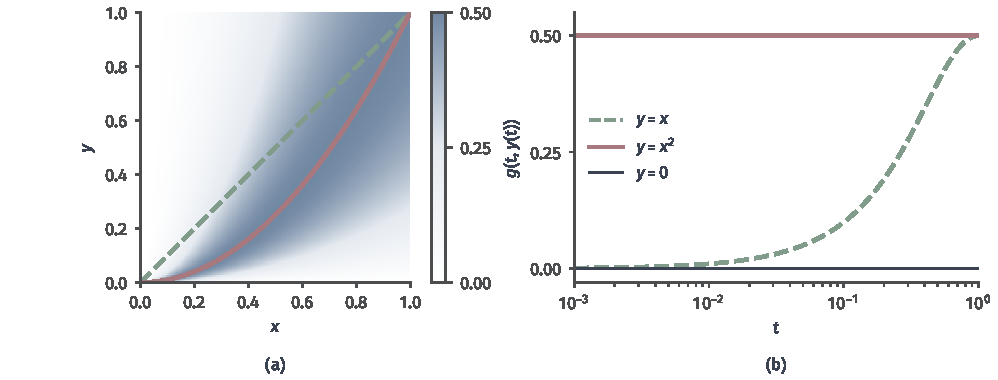
\includegraphics[width=169.0mm]{figures/00-shared/mathematical-preliminaries-upper/00-shared/matplotlib/chapter3-concept-processes/joint-limit-paths.pdf}
 \caption{取前例$g(x,y)=x^2y/(x^4+y^2)$，原点另置零。(a) 第一象限的函数值及三条路径，色阶固定为$0$至$1/2$。(b) 沿$y=0$、$y=x$分别趋零，沿$y=x^2$恒为$1/2$；横轴为正参数$t$的对数刻度，向左趋近原点。不同路径极限足以否定联合极限，有限条路径不能反向证明存在。}
 \label{fig:analysis-process-joint-limit-paths}
\end{figure*}

\paragraph{累次极限与联合极限}
另一种常见做法是逐个坐标取极限，称为累次极限。先令$y\to0$、再令$x\to0$，得到
\[
 \lim_{x\to0}\lim_{y\to0}f(x,y).
\]
内层固定$x\neq0$，让$y$单独趋于$0$；得到一个关于$x$的函数后，外层再让$x$趋于$0$。整个过程从不要求两个坐标同时趋近，因此它与联合极限是不同的问题。
对示例~\ref{ex:multivariable-path-limits}中的$f$，固定$x\neq0$时$f(x,y)\to0$，再令$x\to0$仍为$0$；交换次序同样得到$0$。两个次序的累次极限都为$0$，联合极限却不存在。

累次极限的结果还可能依赖取极限的次序。
\begin{example}[两个次序的累次极限不相等]
\label{ex:multivariable-iterated-limits-differ}
在非原点处令$h(x,y)=x^2/(x^2+y^2)$。固定$x\neq0$而令$y\to0$，得到$x^2/x^2=1$；固定$y\neq0$而令$x\to0$，得到$0$。再取外层极限，
\[
 \begin{gathered}
\lim_{x\to0}\lim_{y\to0}h(x,y)=1\\
\lim_{y\to0}\lim_{x\to0}h(x,y)=0.
 \end{gathered}
\]
内层先把一个坐标压到零，相当于先走到某条坐标轴附近，再沿坐标轴靠近原点。$h$在$x$轴上恒为$1$、在$y$轴上恒为$0$，两种次序因而给出不同结果。
\end{example}

两个例子说明：两个次序的累次极限相等，不足以推出联合极限存在；改变次序也可能改变累次极限。

反方向在补充条件下成立。若联合极限$\lim_{(x,y)\to(0,0)}f(x,y)=L$存在，并且对充分接近$0$的每个$x\neq0$，内层极限$\lim_{y\to0}f(x,y)$都存在，则累次极限$\lim_{x\to0}\lim_{y\to0}f(x,y)$也存在且等于$L$。理由是：给定$\varepsilon>0$，取联合极限定义中的$\delta$；当$0<|x|<\delta/2$、$0<|y|<\delta/2$时$|f(x,y)-L|<\varepsilon$，令$y\to0$，内层极限与$L$相差不超过$\varepsilon$。

\paragraph{统一误差估计}
要证明联合极限存在，可以寻找只依赖距离的上界。若$|f(\bm x)-L|$不超过一个只与$\lVert\bm x-\bm a\rVert_2$有关、并随距离趋于零的量，所有路径就同时受到控制。
\begin{example}[用距离上界证明联合极限]
\label{ex:multivariable-distance-bound-limit}
在非原点处考虑$x^2y/(x^2+y^2)$。由$|xy|\leq(x^2+y^2)/2$，有
\[
 \left|\frac{x^2y}{x^2+y^2}\right|
 =|x|\cdot\frac{|xy|}{x^2+y^2}
 \leq \frac{|x|}{2}
 \leq\frac12\sqrt{x^2+y^2}.
\]
给定$\varepsilon>0$，取$\delta=2\varepsilon$，则距离原点小于$\delta$的非原点都满足误差小于$\varepsilon$，因此原点处极限为$0$。

改用极坐标$(x,y)=(r\cos\theta,r\sin\theta)$，同一函数等于$r\cos^2\theta\sin\theta$，绝对值不超过$r$。这个界对所有$\theta$同时成立，给出同样的结论。
\end{example}

极坐标估计有效，关键在于这个界与角度无关。若只固定$\theta$再令$r\to0$，检查的仍然只是直线。
\begin{example}[固定角度的极坐标检验]
\label{ex:multivariable-polar-fixed-angle}
对示例~\ref{ex:multivariable-parabola-path-limit}中的$g$，代入$(x,y)=(r\cos\theta,r\sin\theta)$得到
\[
 g=\frac{r\cos^2\theta\sin\theta}{r^2\cos^4\theta+\sin^2\theta}.
\]
固定$\theta$再令$r\to0$：$\sin\theta\neq0$时分母趋于$\sin^2\theta$而分子趋于$0$，$\sin\theta=0$时函数恒为$0$，结果总是$0$。
但对每个小的$r>0$，可以取满足$\sin\theta=r\cos^2\theta$的角度。此时分子等于$r^2\cos^4\theta$、分母等于$2r^2\cos^4\theta$，函数值恰为$1/2$。这个角度随$r$改变，对应的点$(r\cos\theta,r\sin\theta)$满足$y=r^2\cos^2\theta=x^2$，正好落在抛物线上。
\end{example}

因此用极坐标证明联合极限时，需要一个对全部$\theta$同时成立、并随$r\to0$趋于零的界。

\section{连续性}
\label{sec:multivariable-continuity}

有了联合极限，就可以讨论连续：输入趋近基点时，输出趋于基点处的值。本节先给出连续性的定义，并用一致连续与Lipschitz连续量化误差的传递；再说明连续性在和、积、复合等运算下保持；最后证明闭有界集上的连续函数取到最值、一致连续。

\subsection{连续性的定义}
\label{sec:multivariable-continuity-definition}

有了联合极限，就可以定义连续：输入联合趋近基点时，输出趋于基点处的值。定义形式与一元连续性相同，只是把$|x-a|$换成输入、输出空间中的距离。
\begin{definition}[映射的连续性]
\label{def:multivariable-scalar-continuity}
设$F:D\to W$、$\bm a\in D$。若对每个$\varepsilon>0$都存在$\delta>0$，使
\[
 \bm x\in D,\quad\lVert\bm x-\bm a\rVert<\delta
 \Longrightarrow \lVert F(\bm x)-F(\bm a)\rVert<\varepsilon,
\]
则称$F$在$\bm a$处连续；在$D$上每点连续时称$F$为连续映射，标量输出时也称连续函数。
\end{definition}
条件中允许$\bm x=\bm a$。在聚点处，这等价于联合极限等于$F(\bm a)$；在孤立点处，取足够小的$\delta$使球内只有$\bm a$，定义自动成立。与极限一样，$F$连续当且仅当每个输出分量连续。
几何上，连续意味着曲面在$\bm a$上方没有裂缝或跳跃：从任何方向走近，高度都平稳地接近$f(\bm a)$。
连续函数的每条坐标切片都连续，但反过来不成立：示例~\ref{ex:multivariable-path-limits}中各条切片都连续，函数在原点却不连续。

\subsection{一致连续与Lipschitz连续}
\label{sec:multivariable-uniform-lipschitz}

连续性允许$\delta$随基点改变。有时需要在整个定义域上用同一个$\delta$统一控制误差。
\begin{definition}[一致连续]
\label{def:ls-uniform-continuity}
设$F:D\to W$。若对每个$\varepsilon>0$存在不依赖基点的$\delta>0$，使$\bm x,\bm y\in D$、$\lVert\bm x-\bm y\rVert<\delta$时$\lVert F(\bm x)-F(\bm y)\rVert<\varepsilon$，就称$F$在$D$上\term{一致连续}。
\end{definition}
有时还要给出误差的数量关系：输出的差至多是输入之差的常数倍。
\begin{definition}[Lipschitz连续]
\label{def:ls-lipschitz}
设$F:D\to W$。若存在常数$L\geq0$，使
\[
 \lVert F(\bm x)-F(\bm y)\rVert\leq L\lVert\bm x-\bm y\rVert\qquad(\bm x,\bm y\in D),
\]
就称$F$在$D$上\term{Lipschitz连续}，$L$称为Lipschitz常数。若每点都有一个邻域，使$F$在该邻域与$D$的交上Lipschitz连续，就称$F$\emph{局部Lipschitz连续}。
\end{definition}
Lipschitz连续蕴含一致连续：取$\delta=\varepsilon/L$（$L=0$时任取）即可。反过来不成立：$\sqrt x$在$[0,1]$上连续，第~\ref{sec:multivariable-closed-bounded-continuous}节将说明它一致连续，但$|\sqrt x-\sqrt0|/|x-0|=1/\sqrt x$在$x\to0^+$时无界，没有Lipschitz常数。范数本身是Lipschitz连续的，由反向三角不等式，常数为$1$。这里只说明误差界的含义；第~\ref{chap:multivariate-differentiation}章将用导数求出可微映射的Lipschitz常数。

\subsection{连续性的性质}
\label{sec:multivariable-continuity-properties}

连续性在常用运算下保持。下面逐条检验和、差、数乘、积、商、乘积型运算与复合，再用它们说明求逆在可逆矩阵上连续。

\paragraph{和的连续性}
设$f,g$在$\bm a$处连续。由三角不等式，
\[
 |(f+g)(\bm x)-(f+g)(\bm a)|\leq|f(\bm x)-f(\bm a)|+|g(\bm x)-g(\bm a)|.
\]
给定$\varepsilon>0$，分别取使两个误差都小于$\varepsilon/2$的半径，其中较小的半径就满足$f+g$的连续性要求。

\paragraph{差的连续性}
相减时两项的误差仍按三角不等式相加：$|(f-g)(\bm x)-(f-g)(\bm a)|\leq|f(\bm x)-f(\bm a)|+|g(\bm x)-g(\bm a)|$。取与和相同的半径，即得$f-g$在$\bm a$处连续。

\paragraph{数乘的连续性}
对固定实数$c$，有$|cf(\bm x)-cf(\bm a)|=|c|\,|f(\bm x)-f(\bm a)|$。$c\neq0$时，把$f$的误差控制在$\varepsilon/|c|$以内即可；$c=0$时$cf$是常函数，结论直接成立。

\paragraph{积的连续性}
若$f,g$在$\bm a$处连续，乘积的误差可以拆成两项：
\[
 f(\bm x)g(\bm x)-f(\bm a)g(\bm a)
 =f(\bm x)\bigl(g(\bm x)-g(\bm a)\bigr)+g(\bm a)\bigl(f(\bm x)-f(\bm a)\bigr).
\]
由$f$的连续性，$\bm x$足够靠近$\bm a$时$|f(\bm x)|\leq|f(\bm a)|+1$，第一项的因子$f(\bm x)$有界；两个括号又都趋于零，所以$fg$在$\bm a$处连续。这与一元的乘积极限法则是同一个论证。

坐标函数$\bm x\mapsto x_j$连续，因为$|x_j-a_j|\leq\lVert\bm x-\bm a\rVert_2$。多元多项式由坐标函数和常数经有限次加法与乘法得到，因此连续，例如$x^2+xy+y^2$。

\paragraph{商的连续性}
除法还要防止分母变为零。若再设$g(\bm a)\neq0$，由$g$的连续性，可以取一个小球使其中$|g(\bm x)|>|g(\bm a)|/2$，即$g$在基点附近远离零。于是
\[
 \left|\frac1{g(\bm x)}-\frac1{g(\bm a)}\right|
 =\frac{|g(\bm x)-g(\bm a)|}{|g(\bm x)|\,|g(\bm a)|}
 \leq\frac{2|g(\bm x)-g(\bm a)|}{g(\bm a)^2}\longrightarrow0,
\]
所以$1/g$在$\bm a$处连续，再用积的连续性得到$f/g$连续。分母非零的条件不能省略，否则商在基点没有定义；由此，有理函数在分母非零处连续。

\paragraph{内积与矩阵乘法}
向量值与矩阵值映射的乘积同样保持连续。若$F,G$在$\bm a$处连续，取值为同维向量，则$\bm x\mapsto F(\bm x)^\top G(\bm x)$在$\bm a$处连续；若$F,G$取矩阵值且形状相容，则$\bm x\mapsto F(\bm x)G(\bm x)$在$\bm a$处连续。理由是结果的每个元素都是有限个分量乘积之和，由和与积的连续性及逐分量判据得到。

\paragraph{复合映射}
若$F:D\to W$在$\bm a$处连续，映射$G$在$F(\bm a)$处连续，且$F$在$\bm a$附近的输出都在$G$的定义域内，则$G\circ F$在$\bm a$处连续。
证明分两步控制误差。给定$\varepsilon>0$，先由$G$的连续性取$\eta>0$，使中间值与$F(\bm a)$相差小于$\eta$时，$G$的输出误差小于$\varepsilon$；再由$F$的连续性取$\delta>0$，使输入距离小于$\delta$时，$F$的输出与$F(\bm a)$相差小于$\eta$。合并两步，$\lVert\bm x-\bm a\rVert<\delta$时就有$\lVert G(F(\bm x))-G(F(\bm a))\rVert<\varepsilon$。
例如$e^{-(x^2+y^2)}$和$\sqrt{1+x^2+y^2}$都是一元连续函数与多项式的复合，因而在整个平面上连续。

\paragraph{逆映射}
矩阵的函数也可以用这些规则检验。记$\mathcal G=\{\bm X\in\mathbb R^{n\times n}:\det\bm X\neq0\}$。由定理~\ref{thm:ls-adjugate-identity}，在$\mathcal G$上
\[
 \bm X^{-1}=\frac{\operatorname{adj}(\bm X)}{\det\bm X}.
\]
$\det\bm X$与$\operatorname{adj}(\bm X)$的每个元素都是$\bm X$各元素的多项式，因而连续；在$\mathcal G$上分母非零，由商的连续性，$\bm X^{-1}$的每个元素都连续。由逐分量判据，求逆$\bm X\mapsto\bm X^{-1}$在可逆矩阵集合上连续。

\subsection{闭有界集上的连续函数}
\label{sec:multivariable-closed-bounded-continuous}

连续性的一个重要用途是保证最值存在。机器学习中常在一块参数区域内最小化损失；如果最小值根本取不到，“求最小点”就没有对象。
一元情形中，闭区间上的连续函数一定取到最值，关键事实是闭区间内任意点列都有收敛于该区间内的子列。第~\ref{sec:multivariable-bolzano-weierstrass-section}节已把这一子列性质推广到有限维闭有界集（定理~\ref{thm:multivariable-bolzano-weierstrass}），本小节用它得到多元极值定理和一致连续性。矩阵空间把元素排成向量后是$\mathbb R^{mn}$，结论相同。

\paragraph{有界性与极值达到}
要让上、下确界由定义域内的点取得，必须防止函数值趋近确界的输入序列逃出定义域。这样的序列可能跑向无穷远，也可能趋向一个不属于定义域的边界点。闭有界集的子列性质同时排除了这两种情况。
\begin{theorem}[闭有界集上的极值定理]
\label{thm:multivariable-extreme-value}
\phantomsection\label{thm:ls-extreme-value}
设$K\subseteq\mathbb R^d$非空、闭且有界，$f:K\to\mathbb R$连续，则$f$有界，且存在$\bm x_{\min},\bm x_{\max}\in K$满足
\[
 f(\bm x_{\min})\leq f(\bm x)\leq f(\bm x_{\max})\qquad(\bm x\in K).
\]
\end{theorem}
\begin{proof}
一元闭区间上最值定理的证明只用到两件事：定义域内任意点列有收敛于定义域内的子列，以及函数连续。
这里的$K$由定理~\ref{thm:multivariable-bolzano-weierstrass}满足同一子列条件，输出仍为实数，所以该证明逐字适用。例如对最大值，取$\bm x_n\in K$使$f(\bm x_n)$趋于上确界，选出收敛子列$\bm x_{n_k}\to\bm x_{\max}\in K$，连续性给出$f(\bm x_{\max})$等于上确界。
\end{proof}
定理的条件只是充分条件，但删去其中任何一个，结论都可能失败。与一元情形一样，可以逐项构造反例。
\begin{example}[删去闭性、有界性或连续性时最值可能取不到]
\label{ex:multivariable-extreme-value-failures}
在开单位圆盘$\{x^2+y^2<1\}$上，连续函数$f(x,y)=x^2+y^2$的上确界为$1$，但趋近上确界的点跑向不属于圆盘的边界圆，最大值取不到；这说明不能删去闭性。
在闭而无界的整个平面上，$f(x,y)=-(x^2+y^2)$在远处无限变小，没有下界；这说明不能删去有界性。
在闭单位圆盘上，令$f(x,y)=x^2+y^2$（$x^2+y^2<1$），并在边界圆上令$f=0$。定义域闭且有界，但$f$在边界圆上不连续，上确界$1$仍取不到；这说明不能删去连续性。
\end{example}

\paragraph{一致连续性}
一元情形中，闭区间上的连续函数一致连续。同样，闭有界集上的连续映射一致连续（定义~\ref{def:ls-uniform-continuity}），证明仍然只用子列性质。
\begin{theorem}[闭有界集上的一致连续性]
\label{thm:multivariable-uniform-continuity}
设$K\subseteq\mathbb R^d$非空、闭且有界，$F:K\to W$连续，则$F$在$K$上一致连续。
\end{theorem}
\begin{proof}
若不然，存在$\varepsilon_0>0$，使每个$\delta=1/n$都对应$\bm x_n,\bm y_n\in K$，满足$\lVert\bm x_n-\bm y_n\rVert<1/n$而$\lVert F(\bm x_n)-F(\bm y_n)\rVert\geq\varepsilon_0$。由定理~\ref{thm:multivariable-bolzano-weierstrass}取收敛子列$\bm x_{n_k}\to\bm x\in K$，则$\lVert\bm y_{n_k}-\bm x\rVert\leq\lVert\bm y_{n_k}-\bm x_{n_k}\rVert+\lVert\bm x_{n_k}-\bm x\rVert\to0$。由$F$在$\bm x$处连续，$F(\bm x_{n_k})$与$F(\bm y_{n_k})$都趋于$F(\bm x)$，两者之差趋于零，与$\varepsilon_0$矛盾。
\end{proof}
第~\ref{chap:region-integrals}章的Riemann和、参数积分与换元，都要在整个区域上统一控制局部近似的误差，用到的正是一致连续性。

\section{矩阵范数与商范数}
\label{sec:ls-derived-norms}

有了范数与前几节的结论，就可以在由已有空间构造出的新空间上定义范数。矩阵（线性映射）组成的空间上，诱导矩阵范数衡量最大放大倍数；商空间上，商范数衡量忽略一个子空间中的差别以后剩下的大小。两者都是定义，它们的上确界或下确界有限、可以取到，用的正是范数等价、闭有界集上的最值与子空间的闭性。线性泛函组成的对偶空间上的对偶范数，放到第~\ref{chap:dual-spaces}章与对偶空间一起讨论。

\subsection{矩阵范数}
\label{sec:ls-matrix-norms}
\label{sec:ch06-map-comparison}
\label{sec:matrix-analysis-norms-effective-rank}
\label{sec:multivariable-operator-norm}

第~\ref{chap:linear-operations}章用Frobenius范数衡量矩阵元素的总体大小。误差分析更常用另一种大小：把矩阵看作映射$\bm x\mapsto\bm A\bm x$，问它最多把输入放大多少倍。

\paragraph{诱导矩阵范数}
设$\bm A\in\mathbb R^{m\times d}$，在$\mathbb R^d$上取输入范数$\lVert\cdot\rVert_\alpha$，在$\mathbb R^m$上取输出范数$\lVert\cdot\rVert_\beta$，两者可以是任意范数。
\begin{definition}[由向量范数诱导的矩阵范数]
\label{def:matrix-analysis-induced-norm}
$\bm A$的\term{诱导矩阵范数}（induced matrix norm）为
\[
 \lVert\bm A\rVert_{\alpha\to\beta}
 =\sup_{\lVert\bm x\rVert_\alpha\leq1}\lVert\bm A\bm x\rVert_\beta .
\]
两端采用同一类$p$范数时简写为$\lVert\bm A\rVert_p$。
\end{definition}
$d\geq1$时，由齐次性，上确界也等于$\sup_{\bm x\neq\bm0}\lVert\bm A\bm x\rVert_\beta/\lVert\bm x\rVert_\alpha$：单位球内的非零$\bm x$满足$\lVert\bm A\bm x\rVert_\beta\leq\lVert\bm A(\bm x/\lVert\bm x\rVert_\alpha)\rVert_\beta$，零向量的贡献为零。定义域为零空间时规定范数为零。

下面先证明这个上确界有限，并由此得到线性作用的连续性。

\subsubsection{线性作用的连续性}
\label{sec:ls-linear-action-continuity}

把矩阵作用看作映射$\bm x\mapsto\bm A\bm x$，诱导范数正是它放大输入的倍数上界，因而也给出连续性的定量形式。
\begin{theorem}[线性作用的连续性]
\label{thm:ls-linear-map-continuity}
设$\bm A\in\mathbb R^{m\times d}$，$\mathbb R^d$与$\mathbb R^m$上分别取范数$\lVert\cdot\rVert_\alpha$与$\lVert\cdot\rVert_\beta$，则：
\begin{enumerate}
 \item 诱导范数$\lVert\bm A\rVert_{\alpha\to\beta}$有限，并且对一切$\bm x$有$\lVert\bm A\bm x\rVert_\beta\leq\lVert\bm A\rVert_{\alpha\to\beta}\lVert\bm x\rVert_\alpha$；
 \item $\bm x\mapsto\bm A\bm x$是Lipschitz连续的：$\lVert\bm A\bm x-\bm A\bm y\rVert_\beta\leq\lVert\bm A\rVert_{\alpha\to\beta}\lVert\bm x-\bm y\rVert_\alpha$；
 \item 定义中的上确界可以取到：存在$\lVert\bm x^\star\rVert_\alpha\leq1$，使$\lVert\bm A\bm x^\star\rVert_\beta=\lVert\bm A\rVert_{\alpha\to\beta}$。
\end{enumerate}
\end{theorem}
\begin{proof}
第一条。把$\bm A\bm x$按列展开，由三角不等式与齐次性，
\[
 \lVert\bm A\bm x\rVert_\beta=\Bigl\lVert\sum_jx_j\bm A\bm e_j\Bigr\rVert_\beta\leq\sum_j|x_j|\,\lVert\bm A\bm e_j\rVert_\beta\leq\Bigl(\max_j\lVert\bm A\bm e_j\rVert_\beta\Bigr)\lVert\bm x\rVert_1 .
\]
由范数等价，存在常数$c$使$\lVert\bm x\rVert_1\leq c\lVert\bm x\rVert_\alpha$，所以$\lVert\bm A\bm x\rVert_\beta\leq C\lVert\bm x\rVert_\alpha$，其中$C=c\max_j\lVert\bm A\bm e_j\rVert_\beta$。于是单位球上的$\lVert\bm A\bm x\rVert_\beta$不超过$C$，上确界有限。对$\bm x\neq\bm0$，$\bm x/\lVert\bm x\rVert_\alpha$在单位球上，由齐次性得所述不等式；$\bm x=\bm0$时两边都为零。

第二条。把第一条用于$\bm x-\bm y$，并利用$\bm A\bm x-\bm A\bm y=\bm A(\bm x-\bm y)$即得。

第三条。单位球$\{\bm x:\lVert\bm x\rVert_\alpha\leq1\}$是闭集，由范数等价又是有界集。函数$\bm x\mapsto\lVert\bm A\bm x\rVert_\beta$是连续的矩阵作用与连续的范数的复合，由极值定理~\ref{thm:multivariable-extreme-value}，它在单位球上取到最大值。
\end{proof}
第一条说明，诱导范数是使$\lVert\bm A\bm x\rVert_\beta\leq C\lVert\bm x\rVert_\alpha$对全部$\bm x$成立的最小常数：比它小的常数在取到最大值的$\bm x^\star$处就不成立。第二条按定义~\ref{def:ls-lipschitz}把这个常数读作误差放大的上界：输入相差$\lVert\bm x-\bm y\rVert_\alpha$时，输出至多相差它的$\lVert\bm A\rVert_{\alpha\to\beta}$倍。第三条使定义中的$\sup$可以写成$\max$。

\paragraph{线性映射的算子范数}
对有限维赋范空间之间的线性映射$T:V\to W$，同样定义\term{算子范数}（operator norm）
\[
 \lVert T\rVert=\sup_{\lVert\bm v\rVert_V\leq1}\lVert T\bm v\rVert_W .
\]
选定$V,W$的基，并把$V,W$原有的范数搬到坐标空间（第~\ref{sec:ls-normed-space-definition}节借助坐标定义范数的方法），$T$由矩阵$\bm A$表示，而$\lVert T\rVert$恰等于$\bm A$在这两个坐标范数下的诱导范数。由定理~\ref{thm:ls-linear-map-continuity}，算子范数有限并可以取到，有限维空间之间的线性映射都Lipschitz连续。换基而保持原空间的范数时，数值不变；若改为在坐标上指定另一种范数，就改变了大小的计量规则。

\subsubsection{常用的诱导范数}
\label{sec:ls-common-induced-norms}

诱导范数与把矩阵看作元素数组的Frobenius范数不同。常用的诱导范数有三种。

前两种可以直接从元素算出：
\[
 \begin{gathered}
 \lVert\bm A\rVert_1=\max_j\sum_i|a_{i,j}|,\\
 \lVert\bm A\rVert_\infty=\max_i\sum_j|a_{i,j}|,
 \end{gathered}
\]
即最大绝对列和与最大绝对行和，推导见下面的“列和与行和公式”。

第三种是诱导$2$范数，也称\term{谱范数}（spectral norm），
\[
 \lVert\bm A\rVert_2=\sup_{\lVert\bm x\rVert_2=1}\lVert\bm A\bm x\rVert_2,
\]
它等于最大奇异值，计算要用到第~\ref{chap:singular-value-decomposition}章的奇异值分解。下面在同一个矩阵上比较两种诱导范数与Frobenius范数。
\begin{example}[同一矩阵在不同口径下的大小]
\label{ex:ls-matrix-norms-shear}
以剪切矩阵
\[
 \bm A=\begin{bmatrix}1&1\\0&1\end{bmatrix}
\]
为例。按列和公式，两列的绝对值之和分别为$1+0=1$与$1+1=2$；按行和公式，两行的绝对值之和分别为$1+1=2$与$0+1=1$；Frobenius范数则把全部元素的平方相加，得$1+1+0+1=3$。所以
\[
 \begin{gathered}
 \lVert\bm A\rVert_1=\max\{1,2\}=2,\\
 \lVert\bm A\rVert_\infty=\max\{2,1\}=2,\\
 \lVert\bm A\rVert_{\mathrm F}=\sqrt3.
 \end{gathered}
\]
$\lVert\bm A\rVert_1$与$\lVert\bm A\rVert_\infty$在这里碰巧相等，但分别由第二列和第一行取得，回答的是不同输入范数下的最大放大倍数；Frobenius范数只汇总元素大小，又给出另一个数值。谈论矩阵“多大”时，须说明所用的口径。
\end{example}
谱范数也有直观的几何意义。如图~\ref{fig:ls-induced-norm-action}，单位圆被$\bm A$拉成椭圆，椭圆最长半轴的长度就是最大放大倍数。
\begin{figure*}[htbp]
  \centering
  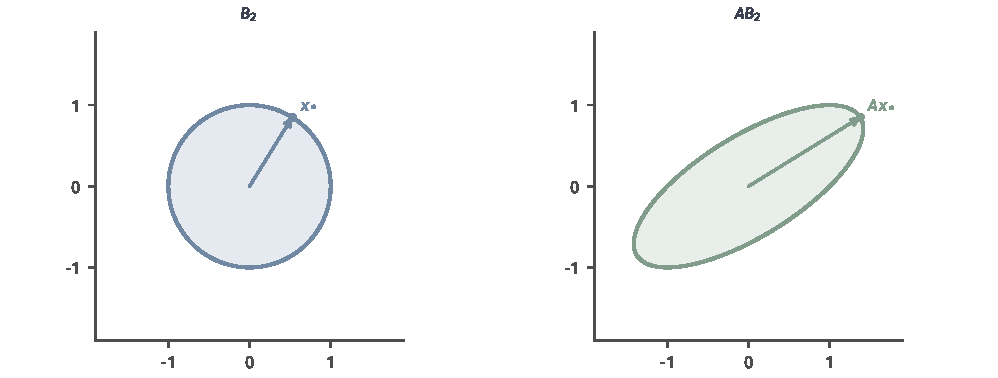
\includegraphics[width=169mm]{figures/00-shared/mathematical-preliminaries-upper/02-linear-spaces/matplotlib/ls-induced-norm-action/ls-induced-norm-action.pdf}
  \caption{诱导矩阵范数衡量最坏放大倍数。左：单位圆$\lVert\bm x\rVert_2=1$；中：线性作用$\bm A$把单位圆映成椭圆；右：椭圆最长的半轴长度就是$\lVert\bm A\rVert_2$，箭头指示最大放大方向。数值由$\bm A$的教学构造直接得到，是解析例。}
  \label{fig:ls-induced-norm-action}
\end{figure*}

\subsubsection{矩阵范数的性质}

有限性与可达性已由定理~\ref{thm:ls-linear-map-continuity}得到。本小节依次求出具体公式、核对范数公理，再给出乘积的上界；这些显式估计用于计算实际的误差常数。

\paragraph{列和与行和公式}
第一式按列计算：
\[
 \lVert\bm A\bm x\rVert_1=\Bigl\lVert\sum_jx_j\bm A_{:,j}\Bigr\rVert_1\leq\sum_j|x_j|\,\lVert\bm A_{:,j}\rVert_1\leq\Bigl(\max_j\lVert\bm A_{:,j}\rVert_1\Bigr)\lVert\bm x\rVert_1.
\]
取$\bm x$为最大绝对列和所在列对应的标准坐标向量时，等号成立。第二式按行计算：对每个$i$，
\[
 |(\bm A\bm x)_i|\leq\sum_j|a_{i,j}|\,|x_j|\leq\Bigl(\sum_j|a_{i,j}|\Bigr)\lVert\bm x\rVert_\infty,
\]
对$i$取最大值即得上界。取输入各坐标为最大绝对行和那一行元素的符号（元素为零处取$1$），等号成立。

\paragraph{谱范数不超过Frobenius范数}
谱范数需要奇异值才能精确计算，但Frobenius范数给出一个容易计算的上界：
\[
 \begin{gathered}
 \lVert\bm A\bm x\rVert_2\leq\lVert\bm A\rVert_{\mathrm F}\lVert\bm x\rVert_2,\\
 \lVert\bm A\rVert_2\leq\lVert\bm A\rVert_{\mathrm F}.
 \end{gathered}
\]
对每行用$p=q=2$的Hölder不等式，得$(\bm A\bm x)_i^2=(\bm A_{i,:}\bm x)^2\leq\lVert\bm A_{i,:}\rVert_2^2\lVert\bm x\rVert_2^2$。对$i$求和，右侧的$\sum_i\lVert\bm A_{i,:}\rVert_2^2$正是$\lVert\bm A\rVert_{\mathrm F}^2$，于是得到第一式。第一式说明每个比值$\lVert\bm A\bm x\rVert_2/\lVert\bm x\rVert_2$都不超过$\lVert\bm A\rVert_{\mathrm F}$，由此得到第二式。

\paragraph{诱导范数是范数}
诱导范数满足范数的各条要求。非负性与齐次性由定义直接得到。若$\lVert\bm A\rVert_{\alpha\to\beta}=0$，则每个$\bm A\bm e_j=\bm0$，即$\bm A=\bm0$，这给出正定性。三角不等式来自$\lVert(\bm A+\bm B)\bm x\rVert_\beta\leq\lVert\bm A\bm x\rVert_\beta+\lVert\bm B\bm x\rVert_\beta$，两边除以$\lVert\bm x\rVert_\alpha$再取上确界即得。

\paragraph{次乘性}
诱导范数还能控制乘积。中间范数匹配时，
\[
 \lVert\bm A\bm B\rVert_{\alpha\to\gamma}
 \leq\lVert\bm A\rVert_{\beta\to\gamma}
 \lVert\bm B\rVert_{\alpha\to\beta}.
\]
这只需连续应用两次诱导范数的界：
\[
 \lVert\bm A\bm B\bm x\rVert_\gamma\leq\lVert\bm A\rVert_{\beta\to\gamma}\lVert\bm B\bm x\rVert_\beta\leq\lVert\bm A\rVert_{\beta\to\gamma}\lVert\bm B\rVert_{\alpha\to\beta}\lVert\bm x\rVert_\alpha.
\]
两边除以$\lVert\bm x\rVert_\alpha$再取上确界即得。反复使用可得$\lVert\bm A^k\rVert_p\leq\lVert\bm A\rVert_p^k$。

\paragraph{Frobenius范数与谱范数的混合界}
乘积的Frobenius范数可以用一个因子的谱范数和另一个因子的Frobenius范数控制：
\begin{equation}
\begin{gathered}
\lVert\bm A\bm B\rVert_{\mathrm F}
 \leq\lVert\bm A\rVert_2\lVert\bm B\rVert_{\mathrm F},\\
\lVert\bm A\bm B\rVert_{\mathrm F}
 \leq\lVert\bm A\rVert_{\mathrm F}\lVert\bm B\rVert_2.
\end{gathered}
\label{eq:matrix-analysis-mixed-submultiplicativity}
\end{equation}
第一式按列计算：
\[
 \lVert\bm A\bm B\rVert_{\mathrm F}^2=\sum_j\lVert\bm A\bm B_{:,j}\rVert_2^2\leq\lVert\bm A\rVert_2^2\sum_j\lVert\bm B_{:,j}\rVert_2^2=\lVert\bm A\rVert_2^2\lVert\bm B\rVert_{\mathrm F}^2.
\]
第二式对转置应用第一式：$\lVert\bm A\bm B\rVert_{\mathrm F}=\lVert\bm B^\top\bm A^\top\rVert_{\mathrm F}\leq\lVert\bm B^\top\rVert_2\lVert\bm A^\top\rVert_{\mathrm F}$。转置不改变Frobenius范数，还需要说明$\lVert\bm B^\top\rVert_2=\lVert\bm B\rVert_2$。对固定的$\bm x$，由$p=q=2$的Hölder不等式，$\lVert\bm y\rVert_2=1$时$|\bm y^\top\bm B\bm x|\leq\lVert\bm B\bm x\rVert_2$；$\bm B\bm x\neq\bm0$时取$\bm y=\bm B\bm x/\lVert\bm B\bm x\rVert_2$即取等号。所以
\[
 \lVert\bm B\rVert_2=\sup_{\lVert\bm x\rVert_2=\lVert\bm y\rVert_2=1}|\bm y^\top\bm B\bm x|.
\]
由于$\bm y^\top\bm B\bm x=\bm x^\top\bm B^\top\bm y$，交换$\bm x,\bm y$的角色，同一个上确界也等于$\lVert\bm B^\top\rVert_2$。再结合$\lVert\bm A\rVert_2\leq\lVert\bm A\rVert_{\mathrm F}$，可知Frobenius范数也满足次乘性：$\lVert\bm A\bm B\rVert_{\mathrm F}\leq\lVert\bm A\rVert_{\mathrm F}\lVert\bm B\rVert_{\mathrm F}$。

\subsection{商范数}
\label{sec:ls-quotient-norms}

子空间的闭性还可以用来给商空间定义范数。第~\ref{sec:ls-quotient-spaces}节的商空间$V/U$把相差$U$中向量的点看成同一个类$\bm x+U$，那里只建立了线性结构。要度量一个类的大小，自然的选择是类中的点到$U$的距离。这个距离不依赖类中代表元的选取：若$\bm x'=\bm x+\bm u_0$，$\bm u_0\in U$，则$\bm u$遍历$U$时$\bm u-\bm u_0$也遍历$U$，所以$d(\bm x',U)=d(\bm x,U)$。于是可以定义\term{商范数}（quotient norm）
\[
 \lVert\bm x+U\rVert_{V/U}=d(\bm x,U)=\inf_{\bm u\in U}\lVert\bm x-\bm u\rVert .
\]

它满足范数的三条要求。三角不等式：对任意$\bm u,\bm u'\in U$，
\[
 d(\bm x+\bm y,U)\leq\lVert(\bm x-\bm u)+(\bm y-\bm u')\rVert\leq\lVert\bm x-\bm u\rVert+\lVert\bm y-\bm u'\rVert;
\]
取$\bm u,\bm u'$使右侧两项分别任意接近$d(\bm x,U)$与$d(\bm y,U)$，即得$d(\bm x+\bm y,U)\leq d(\bm x,U)+d(\bm y,U)$。齐次性：$c\neq0$时$cU=U$，所以$d(c\bm x,U)=|c|\,d(\bm x,U)$；$c=0$时两边都为零。正定性要求$d(\bm x,U)=0$只在$\bm x+U=U$即$\bm x\in U$时发生，这正是前面由子空间闭性得到的结论。在子空间不一定闭的更一般空间中，同一个公式可能只给出半范数，有限维的结论不能无条件外推。

\paragraph{一般范数下的最近点}
商范数是一个下确界。这个下确界能否取到，就是$U$中是否存在离给定点最近的点。
\begin{theorem}[最近点的存在]
\label{thm:multivariable-nearest-point-existence}
设$V$是有限维赋范空间，$U$是子空间，$\bm x\in V$，则存在$\bm u^\star\in U$，使$\lVert\bm x-\bm u^\star\rVert=d(\bm x,U)$。
\end{theorem}
\begin{proof}
在$U$中取$\bm u_k$，使$\lVert\bm x-\bm u_k\rVert\to d(\bm x,U)$。由$\lVert\bm u_k\rVert\leq\lVert\bm x\rVert+\lVert\bm x-\bm u_k\rVert$，序列$(\bm u_k)$有界。由定理~\ref{thm:multivariable-bolzano-weierstrass}（范数等价使它对任意范数适用），存在收敛子列$\bm u_{k_i}\to\bm u^\star$；由子空间闭性，$\bm u^\star\in U$。范数连续，所以$\lVert\bm x-\bm u^\star\rVert=\lim_i\lVert\bm x-\bm u_{k_i}\rVert=d(\bm x,U)$。
\end{proof}
最近点存在，却可能不唯一。
\begin{example}[反例：$\ell_\infty$范数下最近点不唯一]
\label{ex:ls-linf-nonunique-nearest}
在$\mathbb R^2$上取$\ell_\infty$范数，求点$\bm y=(0,1)^\top$到横轴$U=\operatorname{span}\{(1,0)^\top\}$的最近点。$U$中的点写成$(t,0)^\top$，差向量为$(-t,1)^\top$，于是
\[
 \lVert\bm y-(t,0)^\top\rVert_\infty=\max\{|t|,1\}\geq1,
\]
等号当且仅当$|t|\leq1$时成立。

所以$d(\bm y,U)=1$，而且横轴上整整一段$|t|\leq1$的点$(t,0)^\top$都是最近点。原因在于$\ell_\infty$只看最大坐标：竖直方向的差已经是$1$，水平方向的差只要不超过$1$，就不影响距离。欧氏范数下只有$t=0$达到最小距离，可见最近点是否唯一取决于所用的范数，而不只取决于点和子空间。
\end{example}
加入内积以后，第~\ref{sec:ls-orthogonal-projection}节将证明正交投影给出唯一的最近点。一般范数下的存在性与内积几何下的唯一性，回答的是两个不同的问题。

